\documentclass[11pt, titlepage, fleqn]{report}
\usepackage[utf8]{inputenc}
\usepackage[T1]{fontenc}
\usepackage{graphicx}
\usepackage{hyperref}
\usepackage{listings}
\usepackage{siunitx}
\usepackage[left=3cm, right=2cm, top=3cm, bottom=2cm]{geometry}
\usepackage{hsellogo}
\usepackage{hselfonts}
\usepackage{hselcolor}
\usepackage{hselmath}
\usepackage{amsmath}
\usepackage{siunitx}
\usepackage{parskip}
\usepackage{csquotes}
\usepackage{acronym}
\usepackage{wrapfig}
\usepackage{subcaption}
\usepackage{float}
\usepackage{hyphenat}
\usepackage{microtype}
\usepackage{booktabs}
\usepackage[ngerman, german]{babel}
\usepackage[citestyle=numeric,bibstyle=numeric, sorting = none,
hyperref=true,backref=true,maxcitenames=3,url=true,backend=biber,natbib=true]{biblatex}
\addbibresource{references.bib}
\author{Liebenow, Wozasek}
\date{\textit{<2020-01-26 Sun>}}
\title{Dokumentation HoloOSCv2\\\medskip
\large Dokumentation HoloOSCv2}
\hbadness 1000
\tolerance = 200

\begin{document}
\begin{titlepage}% Deckblattk
	\hsellogo\hfill Projektarbeit % etwa Bachelorarbeit, Masterarbeit
	\par
	\vspace{4cm}
	\noindent\parbox{0.8\textwidth}{\Huge RotaCon - Dokumentation}  
	\vspace{2cm}

	\Large \noindent vorgelegt von:
	\begin{itemize}
		\item Tino Liebenow - Matrikelnummer 7011830
	\end{itemize}
	\vspace{2cm}
	betreut duch\newline
	Dipl.-Ing. (FH) Jörg Strick\newline
	Abgabedatum: 30.01.2020
\end{titlepage}
	\newpage
	\tableofcontents
	\listoffigures% Abbildungsverzeichnis
	\listoftables
    \newpage
    \section*{\Huge Abkürzungsverzeichnis}% Abkürzungen
    \label{sec:Abkürzungsverzeichnis}
    \vspace{1cm}
    \begin{acronym}
		\acro{hsel}[HSEL]{Hochschule Emden Leer}
		\acro{cad}[CAD]{computer-aided design}
		\acro{eeprom}[EEPROM]{electrically erasable programmable read-only memory}
		\acro{eq}[EQ]{Equalizer}
		\acro{ide}[IDE]{Integrated Development Environment}
		\acro{io}[I/O]{Input / Output}
		\acro{tp}[TP]{Tiefpass}
		\acro{usb}[USB]{Universal Serial Bus}
    \end{acronym}
	\newpage
	\chapter{Prolog}
		Hier wird Tino am Ende der Arbeit eine tolle Einleitung hinzaubern, die dei Ausgangslage zu derzeitigen Aktivlautsprechern beschreibt, ähnlich der Idee. Außerdem schreibe ich in männlicher Form etc...\newline
		Außerdem reden wir immer vom AKTIV-Lautsprecher...
	\section{Überblick}
		Überblick über den Aufbau der Dokumentation.\newline
		Diese Dokumentation ist in vier Hauptteile gegliedert. Im Prolog wird die Ausgangssituation geschildert, sowie die Kerngedanken zum RotaCon.
	\section{Ziel}
		was möchte Tino heute eigentlich machen?\newline
		Ziel ist es ein Gerät zur Fernbedienbarkeit von Potentiometern, speziell an Lautsprechern, zu entwickeln. Dabei sollen weder Veränderungen am Lautsprechergehäuse, oder an der Technik vorgenommen werden. Zusätzlich ist eine Diskretisierung der Pegelwerte und deren Visualisierung via LCD-Display angedacht, sodass der Benutzer sichtbare 
		Werte zur Orientierung der aktuellen Einstellung bekommt. 
	\section{Stand der Technik}	
		gibts sowas schon?\newline
		Fernsteuerungen für Pegeleinstellungen sind nicht neu auf dem Markt. Dabei sind zwei Varianten verbreitet, zum Einen besteht die Möglichkeit, den Potentiometer auf der Platine des Lautsprechers auszutauschen, zum Anderen die Integrierung eines Controllers in den Signalweg. Die erste Variante setzt somit die Öffnung des Lautsprechergehäuses sowie Manipulation der Elektronik vorraus. Dies ist nicht nur für den durchschnittlichen
		Lautsprecherbesitzer ein schwieriger Eingriff, sondern hat ebenfalls Einfluss auf diverse Garantieansprüche.\newline
		Die andere Variante beinhaltet keine Veränderungen am Lautsprecher selbst, regelt jedoch nur die Signalpegel zum Lautsprecher hin und nicht den integrierten Verstärker. Somit muss für diese Version der Verstärker stets auf Maximum geregelt sein, dies hat je nach Verstärker Einflüsse auf Soundqualität und Stromverbrauch.
	\chapter{Theorie-Teil}
		Das folgende Kapitel beinhaltet die theoretischen Bestandteile zur Umsetzung der Idee. Diese bilden in ihrer Gesamtheit das Konzept,
		nachdem der Prototyp entwickelt wird.
		\section{Theorie Hardware}
		\label{sec:Theorie Hardware}
			\sloppy \nohyphens{
			Lautstärkeregler sind in den meisten Fällen Potentiometer oder Inkrementalgeber. % [https://de.wikipedia.org/wiki/Lautst%C3%A4rkeregler]
			Diese besitzen in der Regel eine 6mm oder 6.35mm Achse, in D-Form oder geriffelt. Um diese Achse rotieren zu können muss also ein Motor mit einer passenden Kupplung angebracht werden. Für präzise Kontrolle und ausreichendes Drehmoment ist ein Schrittmotor geeignet. Diesen gibt es in verschiedenen Ausfertigungen: Unipolar und Bipolar. Unipolare Schrittmotoren haben vier Phasen und werden nur in einer Richtung von Strom durchflossen. Bipolare polen ihre Magnetfelder durch Umkehrung der Stromrichtung um, sie haben zwei Phasen, erreichen ein höheres Drehmoment und sind durch ihre Funktionsweise etwas aufwendiger anzusteuern. 
			Für eine Schrittmotorsteuerung sind drei Funktionseinheiten notwendig. Diese bestehen aus Mikrocontroller, Steuerschaltung und Treiberstufen. Für dieses Projekt ist ein unipolarer Schrittmotor ausreichend, da keine hohen Drehmomente erreicht werden müssen. Dies hat den Vorteil, dass die Steuerschaltung rein auf Softwarebasis gelegt werden kann. Als Treiber soll eine Darlington-Schaltung für den Motor dienen. Die softwaretechnische Besteuerung ist durch ein Arduino mit integriertem Mikrocontroller angestrebt, dessen Spannungsversorgung von 5V idealer Weise auch für die anderen Komponenten ausreichen soll, sodass ein Betrieb des Gerätes durch USB-Spannungsversorgung ermöglicht wird. Da analoge Drehregler durch eine Minimal- und Maximalstellung begrenzt sind, ist auch der Antrieb des Motors in diesen Bereichen zu stoppen. In erster Linie sollen Endschalter den Potentiometeranschlag erkennen und software-gesteuert die Rotation einstellen. Redundant dazu wird der Stromverbrauch des Schrittmotors durch die Kombination eines nicht-invertierenden Verstäkers und dem Analog-Digital-Wandler vom Mikrocontroller überwacht. Für die Bedienung des Gerätes soll ein Infrarotempfänger mit passender Fernbedienung im Frequenzbereich verwendet werden. Da sich Lautstärkeregler meist nicht sichtbar am Lautsprecher befinden, ein IR-Empfänger jedoch eine quasioptische verbindung vorraussetzt, bieten sich zwei getrennte Gehäuseteile an, die durch ein Kabel verbunden sind. In dem sichtbaren Gehäuse befindet sich zusätzlich das Display.}
		\newpage
		\section{Theorie Software}
		\label{sec:Theorie Software}
			Softwaretechnisch sind drei Bereiche abzudecken, genannt seien die Programmierung des Mikrocontrollers an sich, das Entwerfen eines Platinenlayouts sowie der Entwurf der Gehäuse für den 3D-Druck. Bei der Programmierung des Mikrocontrollers soll beachtet werden, dass die aktuellen Werte der Motorstellung und der dazugehörigen Lautstärkeanzeige gespeichert werden, damit bei jeder Inbetriebnahme die jeweils vorherigen Werte beibehalten bleiben. Die einzige Schnittstelle zum Benutzer ist das Display, daher müssen Fehler, Warnungen und wichtige Informationen auf dem Display abgebildet werden. Alle variablen Funktionen des Gerätes sollen über die Fernbedienung steuerbar sein, also die Steuerung der Lautstärke, aber auch das Aktivieren, bzw. Deaktivieren der Displaybeleuchtung.
		\section{Theorie Mechanik}
			Die Übertragung des Drehmoments vom Motor an den Drehregler des Lautsprechers kann nur stattfinden, wenn der Motor starr gelagert ist. Daher ist das Gehäuse mit Motor und Motorsteuerung zu fixieren. Weiterhin sind Lautstärkeregler an verschiedenen Lautsprechern auch an verschiedenen Positionen, sodass dieses Gehäuse zusätzlich in seiner Position variabel positionierbar sein muss. Einige Lautsprecher mit stärkeren Verstärkern haben zusätzlich Kühlkörper an der Lautsprecherrückseite, aus diesem Grund und der Tatsache, dass eventuell weitere Regler (Phase, TP, EQ) vorhanden sind, ist ein gewisser Abstand zwischen den Gehäusen notwendig. Auch die Positionen der Endanschläge sind nicht überall gleich, das bedeutet, dass auch die Endschalter in ihrer Position variierbar sein müssen.
		\label{sec:Theorie Mecanik}
	\chapter{Praxis-Teil}
	\label{sec:Praxistil}
		Folgendes Kapitel beinhaltet die Beschreibung aller im RotaCon verwendeten Bestandteile, sowie der Software, die zum Entwickeln benutzt wurden.
		Es wird auf die Programmierung des Mikrokontrollers eingegangen, die elektronische Schaltung und der Entwurf der Gehäuse wird erläutert.
		\section{verwendetes Material?}
			\subsection{der Arduino Nano}
			\label{sec:Nano}
				%Arduino Praxiseinstieg 2.3 Seite 23?
				%https://store.arduino.cc/arduino-nano
				Arduino ist eine Open-Source Elektronik Plattform, die aus zwei Teilen besteht. Einem Hardware- und einem Softwareteil. Der Hardware-Teil ist eine Microcontroller-Schaltung mit serieller Schnittstelle. Diese ''Microcontroller-Boards'' gibt es in verschiedenen Ausführungen und unterscheiden sich in ihrer Größe, dem verwendeten Microcontroller und den somit einhergehenden Eigenschaften von Ein- und Ausgängen. Die Eingänge können Daten von Sensoren einlesen, die Ausgänge dienen zur Ansteuerung von Motoren, Dioden,	Relais oder anderen elektronischen Komponenten. Die Spannungsversorgung kann über die USB-Schnittstelle oder externem Netzteil erfolgen. Der im RotaCon verwendete Arduino Nano ist eine Leiterplattenversion von geringer Baugröße und nutzt als Basis den ATmega328. Der Arduino Nano hat insgesamt 22 I/O-Pins, 8 davon können als analoge Eingänge benutzt werden. Die logische Spannung des Nanos beträgt 5V, die maximale Stromstärke pro Pin 40 mA. Mit einer Taktrate von 16 MHz und einem integrierten Speicher (EEPROM) von 1KB ist der Arduino Nano in seinen Funktionen ideal für dieses Projekt.
			\subsection{die Arduino IDE}
			\label{sec:Arduino IDE}
				%gleiche Quellen wie oben
				Die Entwicklungsumgebung der Arduino-Plattform stellt den Softareteil dar und basiert auf Processing, einer stark typisierten Programmiersprache mit integrierter Entwicklungsumgebung. Die Programmiersprache ähnelt C++ und ist darauf ausgelegt ohne tiefgründige Programmierkenntnisse Programme schreiben zu können. Programme dieser IDE werden Sketch genannt. Dieser Sketch wird in der IDE compiliert und kann via USB direkt auf den Speicher des Arduino-Boards geladen werden. Ein in die IDE integrierter serieller Monitor kann die jeweiligen Zustände der Ein- und Ausgänge überwachen und ist ein Hilfsmittel zur Fehlersuche in der Entwicklungsphase.
			\subsection{FreeCAD}
			\label{sec:FreeCAD}
				FreeCAD ist eine parametrische Modellierungsanwendung. 3D-Objekte können mit hoher Päzision modelliert und angeordnet werden. Vorteil gegenüber einer Modellierungsanwendung wie Cinema 4D besteht in der Möglichkeit der Herstellung von Unterlagen zum designten Modell. So können beispielsweise technische Zeichnungen und Montagepläne erstellt werden. Die Anwendung ist ein Open-Source Projekt, daher wird es gemeinschaftlich weiterentwickelt und wächst in seinem Funktionsumfang.
				%https://www.freecadweb.org/wiki/Getting_started/de
				%https://de.wikipedia.org/wiki/CAD#Herstellen_von_Fertigungs-/Herstellungsunterlagen
			\subsection{Cura}
			\label{sec:Cura}
				%https://de.wikipedia.org/wiki/Slicer-Software
				%https://ultimaker.com/download/170/Cura_User-Manual_v1.0.pdf
				Cura ist eine Slicing Software von der Firma Ultimaker. Dieses Programm ist für die Umwandlung von 3D-Objektmodellen in spezifische Druckanweisungen verantwortlich. Dazu wird ein 3D-Modell zu einem Stapel von flachen Schichten umgerechnet beziehungsweise ''zerschnitten''. Zusätzliche Einstellungen für den 3D-Drucker werden vorgegeben, sodass Druckablauf, Temperaturen von Druckbett und Extruder, Filament-Art, 
				Vortriebsgeschwindigkeiten und gegebenenfalls Stützen für den Druck von Überhängen festgelegt sind.
			\subsection{Eagle}
			\label{sec:Eagle}
				%http://dl36mmdz94630.cloudfront.net/uploads/eagle_resources/files/000/002/278/original/step-by-step_tutorial.pdf?1484967932
				Die Software Eagle von Autodesk ist ein Platinen-CAD Programm zum entwerfen von Schaltplänen und Platinenlayouts. Dabei sind zwei Hauptschritte der Bearbeitung auszuführen. Zum Einen die Gestaltung des Schaltplans, dazu bietet Eagle durch Einbinden von Biblitheken annähernd alle erdenklichen 
				Schaltsymbole und Bezeichnungen die für den Entwurf der Schaltung notwendig sind. Zusätzlich können manuell Symbole erstellt werden, falls spezielle unkonventionelle oder eigens entwickelte Elemente verwendet werden.
				Im zweiten Schritt wird das Layout der Platine entworfen, um die Leiterbahnen und Bohrungen passend zu platzieren und dimensionieren.
			\subsection{der Schrittmotor ?}
			\label{sec:Motor}
				%Fachkunde Elektrotechnik Seite 460
				Der im RotaCon verwendete unipolare Schrittmotor \textit{28BYJ-48} hat vier Phasen. Das bedeutet vier Elektromagneten steuern die Bewegung des Dauermagnetrotors. Diese vier Elektromagneten werden durch zwei Spulen realisiert, deren Wicklungen je hälftig aufgeteilt und entgegengesetzt gewickelt sind. Sie sind statisch um den Rotor angeordnet. Die einzelnen Phasen werden nur in einer Richtung von Strom durchflossen und steuern so die Polung der Magneten beziehungsweise die Rotationsrichtung des Motors. Die Versorgungsspannung beträgt 5V und der Wiederstand einer Spule ist mit 50$\Omega$ +- 7\% angegeben. Je nach Einphasensteuerung oder Zweiphasensteuerung ergeben sich daher Ströme von etwa 100mA (zweiphasig), bzw 200mA (einphasig). Bei Schrittmotoren werden im Datenblatt Schrittwinkel und Getriebeübersetzung angegeben. Der hier verwendete Motor hat einen Schrittwinkel von 5,625° bei 64 Schritten angegeben und ein Getriebeverhältnis von 1/64. Daraus ergibt sich, dass eine volle Umdrehung der Motorachse 4096 Schritte benötigt. Diese Winkelangabe bezieht sich auf einen Halbschrittbetrieb, daher ist im Vollschrittbetrieb der Schrittwinkel 11,25° beziehungsweise entspricht eine Achsenumdrehung 2048 Schritte.
		\newpage
		\section{Realisierung der Schaltung}
			\subsection{Motorsteuerung}
				%ULN, Darlington, Motormesswerte der Wiederstände, Berechnung der Ströme und Leistungen
				Eine Darlington-Schaltung ist eine Schaltung aus mehreren Transistoren mit hoher Stromverstärkung und wird zur Schaltung beziehungsweise Steuerung großer Lasten eingesetzt. Dabei können die nötigen Steuerströme gering gehalten werden. Der hier verwendete ULN2003 beinhaltet mehrere Darlinton-Transistoren in einem 
				Gehäuse und Vorraussetzung um die niedrigen Steuerströme des Arduinos zum Treiben des Motors zu verwenden. Gemäß Datenblatt ist die Kollektor-Emitter-Sättigungs-Spannung im leitenden Zustand zwischen 0,9 und 1,3 Volt bei oben angenommenen 100mA bis 200mA.
				\begin{figure}[htbp]
					\centering
					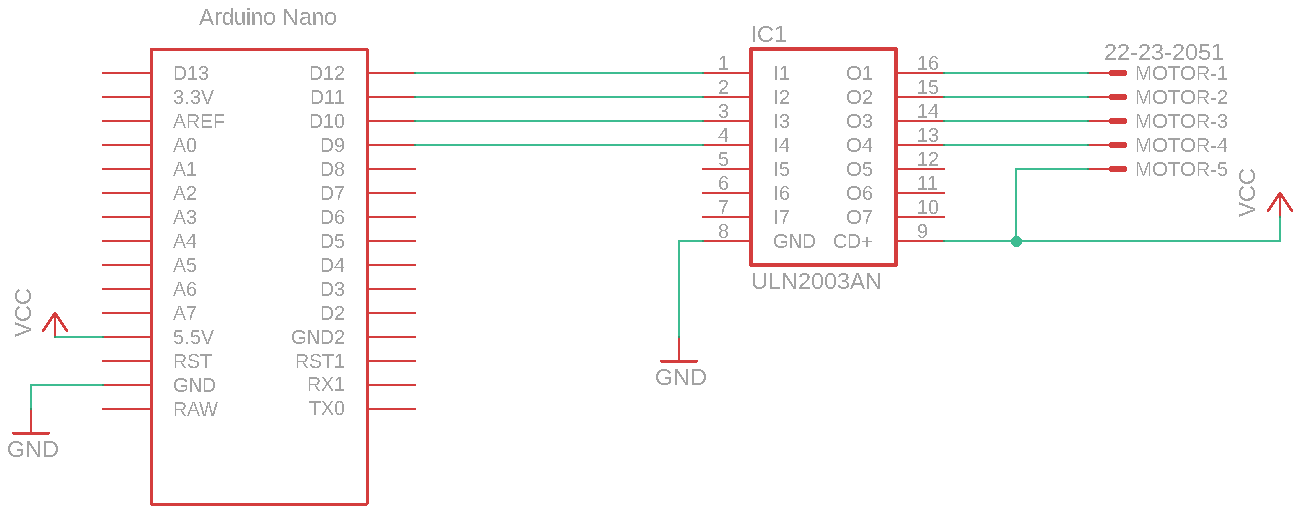
\includegraphics[width=\linewidth]{./img/Motorsteuerung.png}
					\caption{ Ansteuerung des Motors durch Arduino und  Darlington-Transistortreiber ULN2003.
					\label{fig:imgMotorsteuerung}}
				\end{figure}
			\newpage
			\subsection{IR-Receiver}
				%FilterKondensator, FrqBank, Pullup
				Das verwendete Infrarotempfänger-Modul TSOP4838 beinhaltet einen Photosensor, Demodulator und Vorverstärker. Signalpulse mit einer Trägerfrequenz von 38 KHz werden Empfangen, demoduliert, vorverstärkt und an den Output gegeben. Durch den Pullup-Wiederstand wird dieses Signal weiter verstärkt und an den Arduino Nano geleitet. Der analoge Eingang A5 des Arduinos kann als digitaler Eingang betrieben werden und wird hier benutzt um das Platinenlayout übersichtlich zu halten. Zur Filterung von Störsignalen dient der RC-Tiefpass.
				\begin{figure}[htbp]
					\centering
					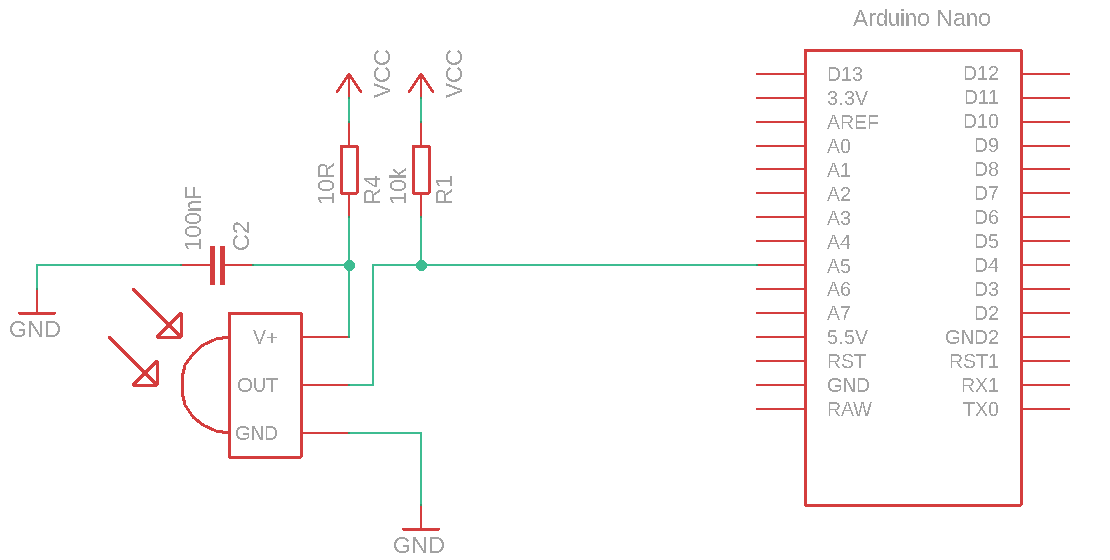
\includegraphics[width=\linewidth]{./img/ir.png}
					\caption{ Infrarot-Empfänger mit Pullup-Wiederstand und Filterkondensator.
					\label{fig:imgIR}}
				\end{figure}
			\newpage	
			\subsection{Display}
				%LCD 16.2, Pinbelegung, Kontrastberechnungl
				Das im RotaCon verwendete LCD-Display ist ein \textit{TC1602B-01}.
				\begin{figure}[htbp]
					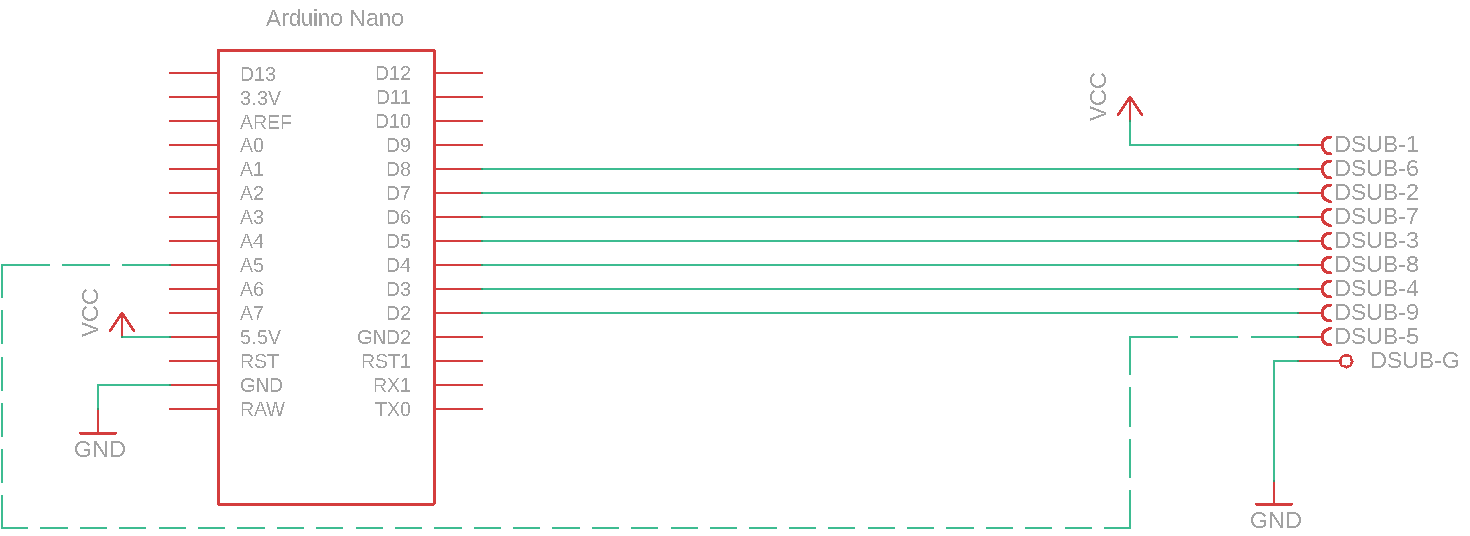
\includegraphics[width=\linewidth]{./img/dsub2.png}
					\label{fig:imgDisplay}
				\end{figure}
			\begin{figure}[htbp]
				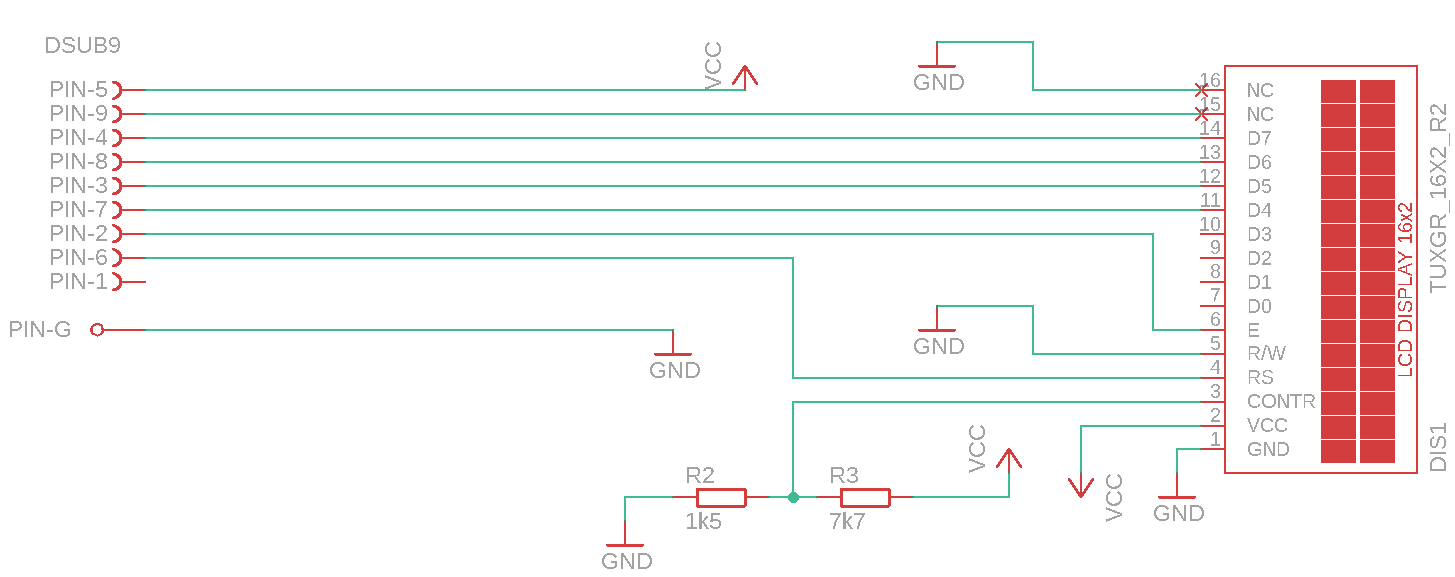
\includegraphics[width=\linewidth]{./img/display2.png}
				\caption{DSUB-Pinbelegung für Display und IR-Receiver(DSUB 5).
				\label{fig:imgDSUB}}
			\end{figure}
			\begin{table}[htbp]
				\caption[Tabelle]{Pin-Belegungen}
				\label{tab:tabDisplay}
				\begin{tabular}{llllllll}
				\toprule
					\textbf{Arduino} & \textbf{DSUB MB} 	  & \textbf{DSUB DB} 	& \textbf{Leiste DB} 	& \textbf{Display}	 & \textbf{Symbol}   & \textbf{Level} & \textbf{Beschreibung}\\
				\midrule
					--		&--		 	  &--			& Pin 1				& Pin 1      & VSS/GND  & 0V    & Ground\\
					--		&--		  	  &--			& Pin 2				& Pin 2      & VDD/VCC  & 5V    & DP Versorgungsspannung\\
					--		&--		 	  &--			& Pin 3				& Pin 3      & V0/CONTR & --    & LCD-Kontrast\\
					D2		& Pin 9		  & Pin 6		& Pin 4				& Pin 4      & RS       & H/L   & H: Datensignal, L: Befehlssignal\\
					--		&--		  	  &--			& Pin 5				& Pin 5      & R/W      & H/L   & H: Lesen, L: Schreiben\\
					D3		& Pin 4		  & Pin 2		& Pin 6				& Pin 6      & E        & H/L   & Enable Display\\
					--		&--		 	  &--			& --				& Pin 7-10	 & D0-D3    & H/L   & Display-Daten\\
					D4		& Pin 8		  & Pin 7		& Pin 7				& Pin 11	 & D4       & H/L   & Display-Daten\\
					D5		& Pin 3		  & Pin 3		& Pin 8				& Pin 12     & D5       & H/L   & Display-Daten\\
					D6		& Pin 7		  & Pin 8		& Pin 9	    		& Pin 13     & D6       & H/L   & Display-Daten\\
					D7		& Pin 2		  & Pin 4		& Pin 10			& Pin 14     & D7       & H/L   & Display-Daten\\
					D8		& Pin 6		  & Pin 9		& Pin 11			& Pin 15     & A        & 5V    & LED-Backlight Anode\\
					--		&--		  	  &--			& Pin 12			& Pin 16     & K		& 0V    & LED-Backlight Kathode\\
					D9		&--		 	  &--			& --				& --     	 & Orange	& H/L   & Motor (Spule 1a)\\
					D10		&--		 	  &--			& --				& --     	 & Gelb		& H/L   & Motor (Spule 2a)\\
					D11		&--		 	  &--			& --				& --    	 & Pink		& H/L   & Motor (Spule 1b)\\
					D12		&--		 	  &--			& --				& --    	 & Blau		& H/L   & Motor (Spule 2b)\\
					A5		& Pin 5		  & Pin 1		& --				& --    	 & --		& H/L   & IR-Receiver\\
					--		& Pin 1		  & Pin 5		& --				& --    	 & VCC		& 5V    & VCC\\
					A0		& --		  &--			& --				& --    	 & --		& 0-5V  & A/D Strommessung Motor\\
					A1		& --		  &--			& --				& --    	 & --		& H/L   & Taster 1\\
					A2		& --		  &--			& --				& --    	 & --		& H/L   & Taster 2\\

				\end{tabular}
			\end{table}
			\newpage
			\subsection{Anschlagerkennung durch Strommessung}
				%OP-Verstärker, Berechnung, vergleich mit Messungen/Erwartungen (TABELLE?)
				LM324N
				\begin{figure}[htbp]
					\centering
					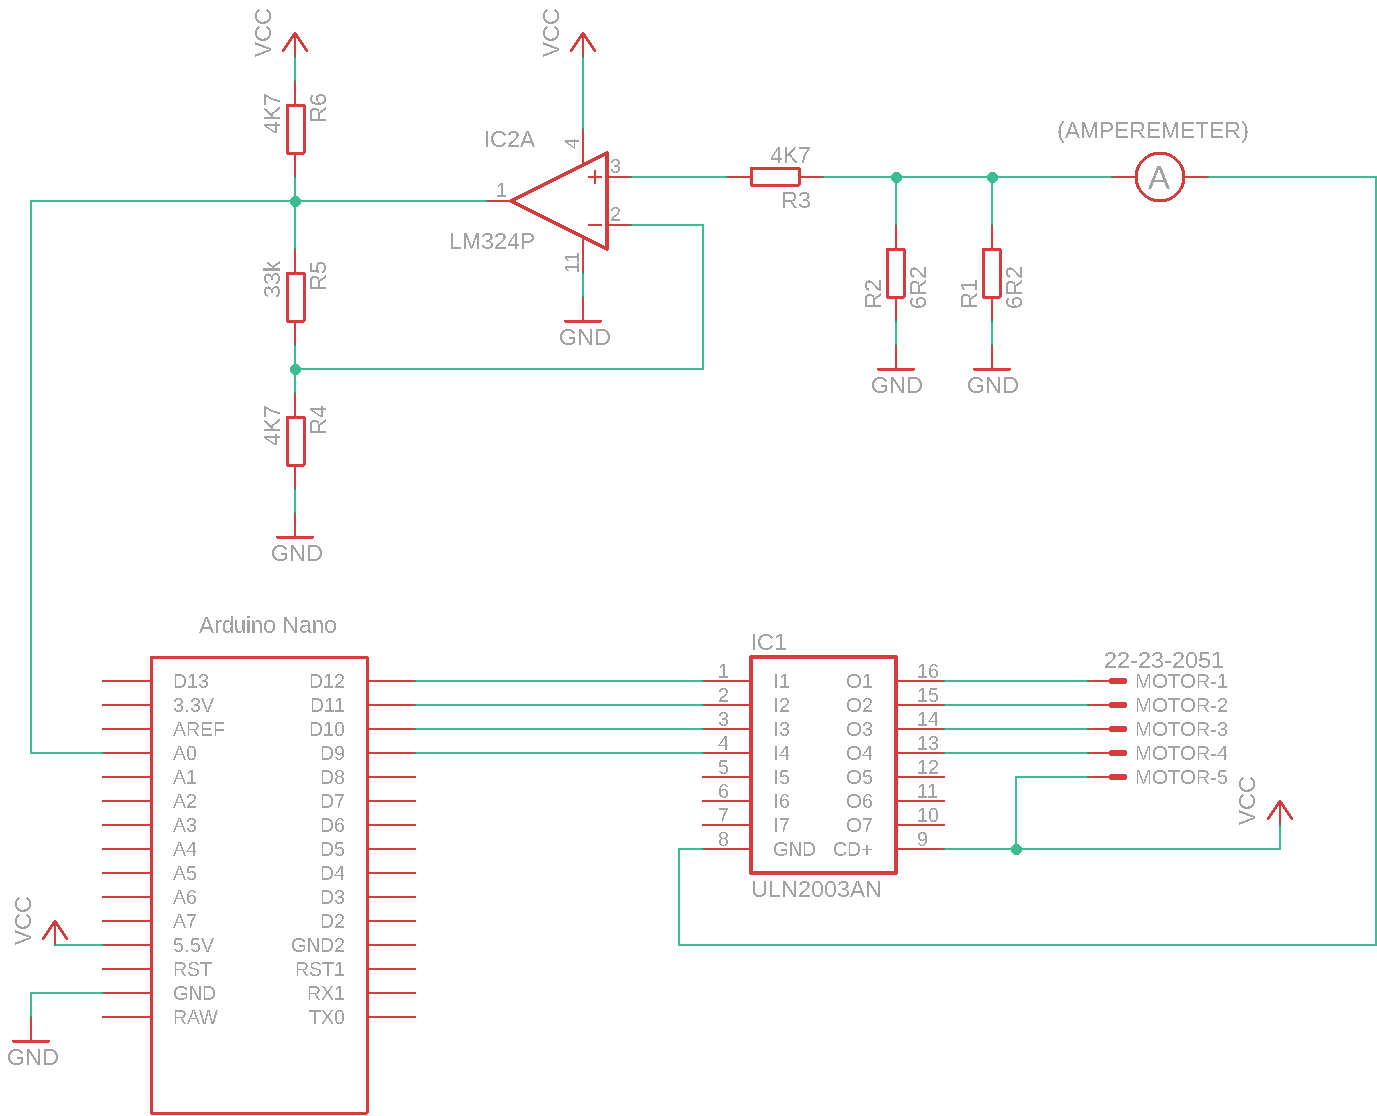
\includegraphics[width=\linewidth]{./img/op2.png}
					\caption{Einsatz eines nicht-invertierenden Verstärkers zur Strommessung.
					\label{fig:imgOP}}
				\end{figure}
			\newpage
			\subsection{Anschlagerkennung durch Endschalter}
				%Redundanz, pullUp
			\subsection{Gesamtschaltung}
				%SChaltpläne eventuell als Beginn des Kapitels?
				%Verbindung der Gehäuse mit DSUB9, Polbelegung DSUB
		\section{Software}
			%Matrizen zur Motorsteuerung, case für IR-auslesen, Messung und Minimalwert
		\section{Das Gehäuse}
			\subsection{Motorgehäuse}
				%Zeichnung, Modell, gesliced, fertigstück ?
				%Besonderheiten/Probleme
			\subsection{Displaygehäuse}
			\subsection{Gehäuseständer}
		\section{Inbetriebnahme / Probleme / Zusammenfassung / Ausblick}
	\chapter{Anhänge}
		\section{Tabelle Teileübersicht}
		\section{Datenblätter}
			Eine Tabelle mit der Auflistung aller Einzelteile mit anschließenden wichtigen Bereichen der Datenblätter.
			Die gesamten Datenblätter werden nicht eingefügt, jedoch ein Link der zu einem derzeitigen Datenblatt im Internet führt.
		\section{Schaltplan}
			Die 2 Schaltpläne der eigenen Platinen.
		\section{Layout}
			Die 2 Platinenlayouts.
		\section{Abmessungen}
			Technische Zeichnungen von FreeCAD mit den Abmessungen der Gehäuse.
		\section{Quellcode}
			Ausschnitte des Quellcodes.
	
\end{document}